\documentclass[]{elsarticle} %review=doublespace preprint=single 5p=2 column
%%% Begin My package additions %%%%%%%%%%%%%%%%%%%
\usepackage[hyphens]{url}

  \journal{Which journal? Journal of Service Research/Health Services Research/EJOR/IJF} % Sets Journal name


\usepackage{lineno} % add
\providecommand{\tightlist}{%
  \setlength{\itemsep}{0pt}\setlength{\parskip}{0pt}}

\usepackage{graphicx}
%%%%%%%%%%%%%%%% end my additions to header

\usepackage[T1]{fontenc}
\usepackage{lmodern}
\usepackage{amssymb,amsmath}
\usepackage{ifxetex,ifluatex}
\usepackage{fixltx2e} % provides \textsubscript
% use upquote if available, for straight quotes in verbatim environments
\IfFileExists{upquote.sty}{\usepackage{upquote}}{}
\ifnum 0\ifxetex 1\fi\ifluatex 1\fi=0 % if pdftex
  \usepackage[utf8]{inputenc}
\else % if luatex or xelatex
  \usepackage{fontspec}
  \ifxetex
    \usepackage{xltxtra,xunicode}
  \fi
  \defaultfontfeatures{Mapping=tex-text,Scale=MatchLowercase}
  \newcommand{\euro}{€}
\fi
% use microtype if available
\IfFileExists{microtype.sty}{\usepackage{microtype}}{}
\usepackage[top=25mm, left=30mm, right=30mm, bottom=25mm,headsep=10mm, footskip=12mm]{geometry}
\usepackage{natbib}
\bibliographystyle{plainnat}
\usepackage{longtable,booktabs,array}
\usepackage{calc} % for calculating minipage widths
% Correct order of tables after \paragraph or \subparagraph
\usepackage{etoolbox}
\makeatletter
\patchcmd\longtable{\par}{\if@noskipsec\mbox{}\fi\par}{}{}
\makeatother
% Allow footnotes in longtable head/foot
\IfFileExists{footnotehyper.sty}{\usepackage{footnotehyper}}{\usepackage{footnote}}
\makesavenoteenv{longtable}
\ifxetex
  \usepackage[setpagesize=false, % page size defined by xetex
              unicode=false, % unicode breaks when used with xetex
              xetex]{hyperref}
\else
  \usepackage[unicode=true]{hyperref}
\fi
\hypersetup{breaklinks=true,
            bookmarks=true,
            pdfauthor={},
            pdftitle={Short-term hourly forecasting for care services},
            colorlinks=false,
            urlcolor=blue,
            linkcolor=magenta,
            pdfborder={0 0 0}}
\urlstyle{same}  % don't use monospace font for urls

\setcounter{secnumdepth}{5}
% Pandoc toggle for numbering sections (defaults to be off)

% Pandoc citation processing

% Pandoc header
\usepackage{adjustbox, float,lscape, bm}
\usepackage{booktabs}
\usepackage{longtable}
\usepackage{array}
\usepackage{multirow}
\usepackage{wrapfig}
\usepackage{float}
\usepackage{colortbl}
\usepackage{pdflscape}
\usepackage{tabu}
\usepackage{threeparttable}
\usepackage{threeparttablex}
\usepackage[normalem]{ulem}
\usepackage{makecell}
\usepackage{xcolor}



\begin{document}
\begin{frontmatter}

  \title{Short-term hourly forecasting for care services}
    \author[University1]{Author1\corref{1}}
   \ead{email1@example.com} 
    \author[University2]{Author2\corref{2}}
   \ead{email2@example.com} 
    \author[Centre for Marketing Analytics and Forecasting, Lancaster University, UK]{Ivan Svetunkov\corref{2}}
   \ead{i.svetunkov@lancaster.ac.uk} 
      \address[University1]{Cardiff business school, 3 Colum Drive, CF10 3EU, Cardiff}
    \address[University2]{adress2}
    \address[University3]{adress3}
      \cortext[1]{Corresponding Author}
    \cortext[2]{Equal contribution}
  
  \begin{abstract}
  The Objective of this work would be to propose a new methodology to forecast short-term hourly forecasting for urgent and emergency care.
  \end{abstract}
  
 \end{frontmatter}

\hypertarget{introduction}{%
\section{Introduction}\label{introduction}}

Demand forecasting is a critical input to inform capacity planning and staffing to meet the needs of patients in each hospital services. An accurate demand forecast contributes to a better decision making process regarding the resources needed to provide services to the number and type of patients requiring hospital services. This is one of the best ways to optimize staffing utilization and related costs. Most current practice to optimise personnel scheduling follows the general approach originally presented in \citep{vile2016time}, which recommends that the following steps be taken to roster employees: (i) forecast demand; (ii) convert demand forecasts into staffing requirements; (iii) schedule shifts optimally; and (iv) assign employees to shifts.

An accurate demand forecasting is crucial in Accident \& Emergency and Ambulance Services in particular to depict various courses of action that can result in massive savings in terms of patient lives.
Unability to match the staff with the demand results in patient overcrowding the in urgent and emergency care system which is a serious problem that causes challenging situations on patient flow. Also, it is related with increasing length of stay, low patient satisfaction, number of patients left the A\&E without seen by staff, unexpected return visits to A\&Es , increasing health care costs, inaccuracy in electronic medical record, and reported waiting times without incurring last-minute expenses, such as overtime or supplemental staffing.

An accurate forecast of the patient demand by hour of the day enables managers to match staff to meet anticipated patients, reconfigure units and redeploy staff. This will have many advantages for both patients, staff and the quality of healthcare services provided.

Furthermore, because the consequences of imperfact staffing are asymmetric probabilistic forecasts are necessary to make economic decicions. This asymmetry arrises because it is preferable to incure a small opportunity cost associated unerutilised staff rather than lower service levels if staff levels are insufficient.

Hourly forecasts are required to inform the short-term operational planning for the current and the upcoming shifts of the day. This involves the short-term decision making related to the execution of the delivery process for various health care services such as Ambulatory, Emergency, Surgical, Inpatient, Home and Residential.

The combination of an hourly forecast demand, incidents being attended, resource availability and delays at hospitals, provide information on the state of the unscheduled care system across the service. Having this full picture enables the delivery managers to focus on the areas that require intervention to enable the most effective delivery of the service to the patients.

Moreover, there are often unplanned events, such as walk-in patients, extended consultation times, during a day or a week. Staff capacities may be adjusted based on the predicted demand fluctuations by using part-time, on-call nurses, staff overtime and voluntary absenteeism. That may also require to adjust the schediling.

what literature says about hourly forecasting in healthcare?

There exists a large literature on demand forecasting of patient needs, however the main focus is on the daily arrivals. Hourly forecasts are challenging because the noise caused by random variation may overshadow any pattern in the data. In this respect, forecasts of daily or monthly arrivals are likely easier but target decisions about staff allocation and the like, not the ongoing scheduling and rescheduling of how the available resources are divided among the patients in need of emergency services

limitations in current literature?
- Typically focus on daily data, hiding information about peak arrival rates. Hourly data has additional challenge of multiple seasonality.
- Deterministic, are there any examples of probabilistic?

Other papers to review and possibly cite:
- Daily visits using Prophet \citet{park2019144}
- Daily using internet data \citet{ekstrom2015forecasting}
- Review paper: \citet{wargon2009systematic}
- Others: \citet{boyle2012predicting},
- Impact of weather \citet{parsons2011modelling}, \citet{macgregor2003effect}

Our contributions are as following:

\begin{enumerate}
\def\labelenumi{\arabic{enumi}.}
\tightlist
\item
  We develop a novel methodology to forecast hourly time series for healthcare services combining a distribution fit to each hour of day separately and then adjust it using variables accounting for i) trend, ii) autocorrelation iii) temporal factors such as day of week, \ldots{} iv) special events such as public holidays, festive days and rugby and v) weather data.
\item
  We provide probabilistic forecasts \ldots{}
\item
  We benchmark the forecasting performance of the proposed methodology against regression, prophet and FASSTER using \ldots.
\item
  We provide data and code enabling reproduction and refinement of the proposed approach
\end{enumerate}

The rest of the paper is organised as following: section \ref{lit} provides a brief overview of hourly forecasting in the healthcare Section \ref{model} starts with \ldots{}

\hypertarget{lit}{%
\section{Research background: Hourly forecasting in care services}\label{lit}}

Table \ref{tab:summarylit} summarise studies in hourly forecasting in emergency and urgent care.

\begin{table}[!h]

\caption{\label{tab:summarylit}Summary of studies in hourly emergency care forecasting}
\centering
\resizebox{\linewidth}{!}{
\begin{tabular}[t]{lrll>{\raggedright\arraybackslash}p{15em}l}
\toprule
Author & Year & Forecast variable & Forecast Horizon & Method & Measure\\
\midrule
McCarthy 
2008 & 2008 & ED arrivals & 24h & Poisson log-linear regression model, including temporal factors, patient characteristics and climatic factors & 95\% CI\\
Asheim et al. & 2019 & ED arrivals & 3h & Poisson regression with weekly and yearly cyclic 
effects. & MAPE\\
Cote et al. & 2013 & ED arrivals & 24h & Fourier regression & R\textasciicircum{}2,  Standard Error\\
Kim et al. & 2014 & Hospital demand & 4h, 24h, 7days, 
30days & Linear regression; Exponential smoothing; ARIMA; GARCH; VAR & MAPE\\
Schweigler et al. & 2009 & ED bed occupancy & 4h and 12h & Hourly historical average; SARIMA; Sinusoidal model with autocorrelated error & RMSE\\
Channouf et al. & 2007 & Ambulance demand & 12h,14h,17h,23h,24h,1h,3h,6h, 13h & Regression & RMSE\\
Hertzum & 2017 & ED arrivals
ED occupancy & 1,2,4,8,24 hours & linear regression; SARIMA; Naïve & MAE, MAPE, 
MASE\\
Choudhury and Urena & 2020 & ED arrivals & 1h to 24h & ARIMA; Holt-winters; TBATS; ANN & RMSE, ME\\
Steins et al. & 2019 & Ambulance call & 24h & ZIP and ZINB regression;
 moving average with seasonality weights & ME, MAE, RMSE\\
Jones et al. & 2009 & ED census & 24h & VAR;  Holt winters & MAE\\
Morzuch and Allen & 2006 & ED arrivals & 168h & Regression; ARIMA; Exponential smoothing & RMSE\\
Chase et al. & 2012 & ED CUR & 30m
1h, 2h, 4h, 8h, 12h & Binary regression & NA\\
Taylor & 2008 & centre volume & 30 minutes 
to 2 weeks & ARMA, Exponential smoothing; Dynamic harmonic regression; Seasonal random walk; Seasonal mean;
Random walk; Mean; Median; Simple exponential smoothing & MAE
RMSE\\
Gijo and Balakrishna & 2016 & call volume & 168h & SARIMA & MMSE\\
\bottomrule
\end{tabular}}
\end{table}

Linear regression, ARIMA, and naive models were used by \citet{hertzum2017forecasting} to investigate whether accurate hourly accident and emergency department patient arrivals and occupancy forecasts can be generated using calendar variables. Naive model was there for the purpose of comparison. \citet{hertzum2017forecasting} study shows that patient arrivals variation is larger across the hours of the day than across the days of the week and the months of the year. In term of hour of the day, patient arrivals peaked around noon. For days of the week, Monday is the busiest day while weekends are the quietest days. July-August are the month with the highest number of patient arrivals and January and February are the months with the lowest number of arrivals. The regression and ARIMA models perform similarly for all forecast interval in modeling patient arrivals. In modeling accident and emergency department occupancy, ARIMA outperform regression models. However, after all, the models of occupancy were less accurate than those arrivals. \citet{hertzum2017forecasting} mentioned that ARIMA models are among the most accurate models for accident and emergency department visits forecasting. Another interesting point is that the accuracy of accident and emergency department forecasting models decrease with the increasing forecast interval. Lastly, the accuracy of the forecasting model may possibly be increased with additional information added to the model.

Predicting the arrivals of accident and emergency department future patients is studied by \citet{choudhury2020forecasting} ARIMA, Holt-Winters, TBATS, and neutral network methods were implemented to forecast hourly accident and emergency department arrivals. ARIMA model was selected as the best fit model and it has provided high and acceptable hourly accident and emergency department forecasting accuracy. \citet{hertzum2017forecasting} work was mentioned in this paper. It is said that residual normality, stationarity, and autocorrelation have not been tested in \citet{hertzum2017forecasting} paper and this might be the cause of accuracy problems. However, residual normality, stationarity, and autocorrelation are tested and compared with Holt-Winters, TBATS, and neutral network methods in \citet{choudhury2020forecasting}
\citet{morzuch2006forecasting} use the Unobserved Components Model (UCM), by which each component of the time series is separately modelled as stochastic; double-seasonal exponential smoothing and standard Holt-Winters to forecast ED arrival for an horizon of 168 hours. The hourly data collected from an Emergency department in Pennsylvania showed no trend, and two seasonal cycles: a within-day and a within-week seasonal cycles. The double seasonal model recorded lower RMSEs for all the 168-hour horizons, which was expected due to the strong hourly seasonality of the time series.

\citet{mccarthy2008challenge} predict patient demand for ED services by characterising ED arrivals. Hourly arrival data of ED arrivals in the 1-year study period was deployed to forecast from 1 hour to 24 hours into the future. Authors use a Poisson log-linear regression model, including independent variables such as temporal factors (i.e., hour-of-day, day- of-week, type-of-day, season, and calendar year), patient characteristics (i.e., age, gender, insurance status, triage level, mode of arrival, and ambulance diversion status) and climatic factors (i.e., temperature and precipitation).
Then, they presente the predictiona interval accuracy of 50 and \(90\%\) intervals for the number of hourly arrivals under the Poisson assumptions. They show that the most important predictor is hour of the day and autocorrelation lag 1. However, these findings are limited to the short period of data (one year).

\citet{schweigler2009forecasting} conducted an investigation on whether using time series methods could accurately generate short-term forecasts of ED bed occupancy.
A year-long dataset of hourly ED bed occupancy was collected from three facilities. For each facility, the authors implemented an hourly historical average model, SARIMA model and sinusoidal model with autocorrelated error. In particular, the historical average model was based on the mean occupancy for each site for each hour of the day; while the sinusoidal model was based on 4 parameters: an AR term, a sine coefficient, a cosine coefficient and an intercept. They evaluated the forecast accuracy of four and twelve hours forecast horizon using RMSE and they found that both SARIMA and the sinusoidal model outperformed the historical average (for example, at site 2, the two models improved by \(33\%\) the 12-hour forecasts generated by historical average).

\citet{kim2014predicting} compared different univariate and multivariate time series forecasting techniques to forecast patient volume for a Hospital Medicine programme.
The study adopted historical mean linear regression as benchmark, exponential smoothing, ARIMA, SARIMA, GARCH (generalized autoregressive conditional heteroskedasticity method), able to adjust changes in variance over time and vector autoregressive (VAR) method, able to incorporate data from different sources, to forecast for 4 hours, 24 hours. They used MAPE to report the forecast accuracy.
Each of the forecasting models outperformed the benchmark model. In particular, ARIMA model performed best.

\citet{gijo2016sarima} generated a time series model to forecast the daily and hourly call volume at all centre handling emergency ambulance services. Since historical data showed seasonality, SARIMA models were investigated. Regarding the daily model, the authors generated a SARIMA model, which, however, resulted in the forecast error (MMSE) that significantly increased when the lead time exceeded 8 days. On the other hand, the SARIMA model proposed to forecast the log-calls an hourly basis. This model was found to fit well the model both for shorter and longer lead times.

\citet{asheim2019real} developed a Poisson time-series regression model with continuous weekly and yearly cyclic effects to implement a real-time system that could forecast ED arrivals on 1,2,3 hours horizon. Once measured the accuracy using the MAPE metric, it was noticed that great improvement happened when time of notification was incorporated into the model, especially on a one-hour horizon. Therefore, time of patient notification must be available for this model to be successful.

\citet{steins2019forecasting} aimed to develop a forecasting model for predicting the number of ambulance services calls per hour and geographical areas, to support managers in decisions-making and to investigate which ones were the factors that affected the number of calls.
Data collected consisted of a time and location of historical ambulance call data for three counties in Sweden and a list of explanatory factors of the area, such as socioeconomic and geographic.
In order to deal with large number of zeros in the data, authors developed zero-inflated Poisson (ZIP) and zero-inflated negative binomial (ZINB) regression models. These were then compared to the currently existing forecasting system, based on moving average with seasonality weights, using ME, MAE and RMSE. Firstly, the factors affecting the number of ambulance calls were found to be the following: population in different age groups, median income, length of road, number of nightlife spots (the number of restaurants), day of the week and hour of the day. Secondly, it was found that the older population (65-100) generated more ambulance calls and that ZIP model performs better than the current model. However, the improvement provided by the more advance model was not much greater than the one provided by the existing model. Authors suggested that it could be because the population, which was used as an independent variable in both models, was so dominant compared to the other factors.
Moreover, both models either underestimated or overestimated the number of calls. Authors suggested that the inability to capture a positive trend resulted in underestimation, and the opposite was due to a negative trend. Therefore, authors recommended that further research should add certain temporal variables able to capture the trend.

According to the studies mentioned earlier, it can be said that the existing studies have shown complications in forecasting hourly patient accident and emergency department visits and the application of forecasting hourly patients visits is not well established. Some of the studies said that the accuracy of hourly accident and emergency department forecasting model is low compared to other longer forecasting intervals like daily forecast \citep{boyle2012predicting, hertzum2017forecasting}. However, some studies mentioned that the accuracy of accident and emergency department hourly forecast is at the acceptable level \citep{choudhury2020forecasting, mccarthy2008challenge, schweigler2009forecasting}.

The literature review reveals some limitations in forecasting for urgent and emergency care which will be summarised as follows:

\begin{itemize}
\tightlist
\item
  first,
\item
  second,
\item
  third,
\end{itemize}

\hypertarget{design}{%
\section{Experimental design}\label{design}}

\hypertarget{data}{%
\subsection{data}\label{data}}

Figure \ref{fig:hourly-plot}

Figure \ref{fig:hourly-plot-ridge}

\begin{figure}[H]

{\centering 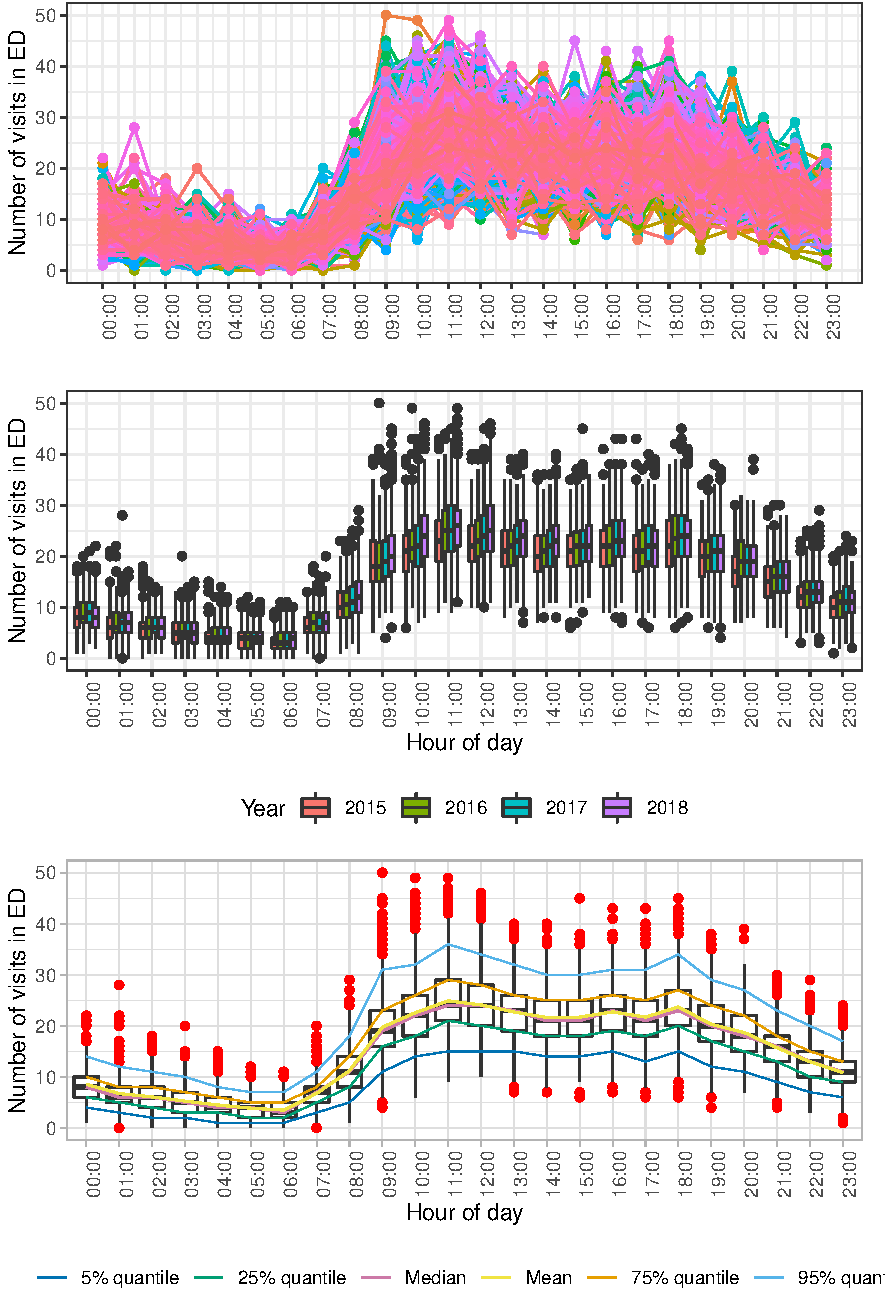
\includegraphics{paper_files/figure-latex/hourly-plot-1} 

}

\caption{Seasonal plot of ED attendance}\label{fig:hourly-plot}
\end{figure}

\begin{figure}[H]

{\centering 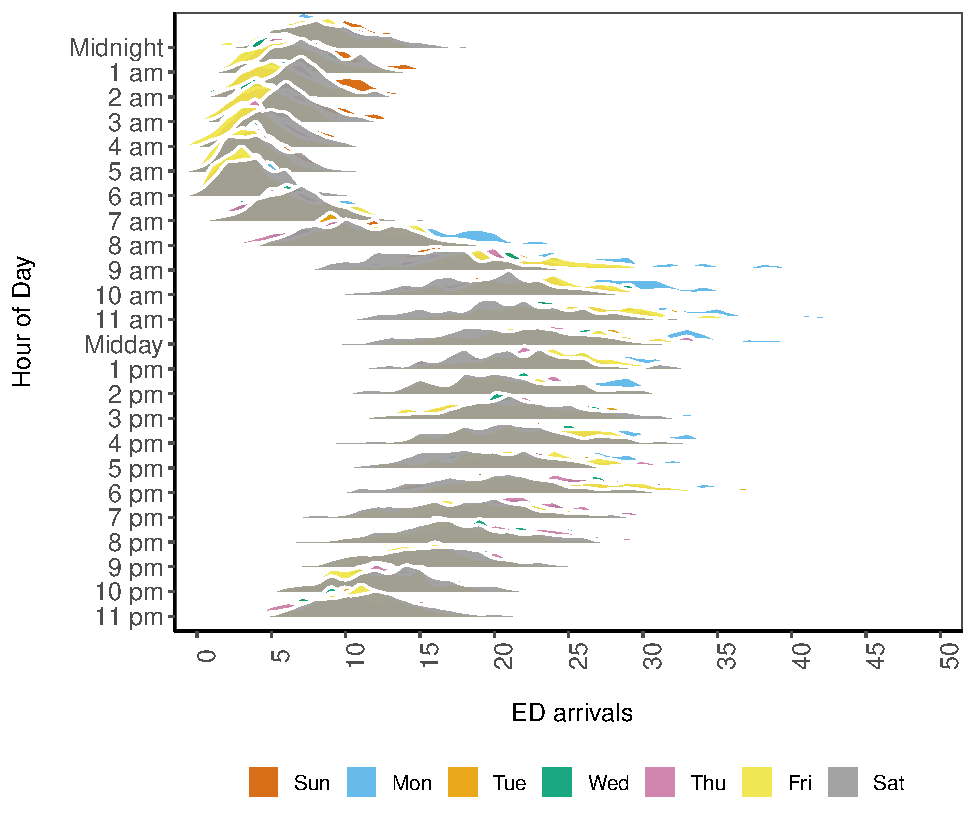
\includegraphics{paper_files/figure-latex/hourly-plot-ridge-1} 

}

\caption{Distrubution of admission per hour and day of the week}\label{fig:hourly-plot-ridge}
\end{figure}

\hypertarget{benchmarks}{%
\subsection{Benchmarks}\label{benchmarks}}

\hypertarget{naiveclimatology}{%
\subsubsection{Naive/Climatology}\label{naiveclimatology}}

Empirical distribution for same hour-of-day and day-of-week as target time.

\hypertarget{multiple-regression}{%
\subsubsection{Multiple Regression}\label{multiple-regression}}

Regression is one of the most popular forecasting methods that uses explanatory variables to predict a variable of interest (in our case, the A\&E admittance). The classical linear regression model is formulated as:

\begin{equation}
  \mathbf{y}_t = \mathbf{x}_t' \boldsymbol{\beta} + \epsilon_t ,
\label{eq:linearRegression}
\end{equation}

where \(\mathbf{x}_t\) is the vector of explanatory variables, \(\boldsymbol{\beta}\) is the vector of parameters and \(\epsilon_t\) is the error term, which is typically assumed to follow Normal distribution with zero mean and a fixed variance. However, in the context of healthcare and A\&E admittance, the assumption of Normality is unrealistic, because the number of admitted patients is integer and non-negative. So the linear regression model should be substituted by some other model. One of the models that is frequently used in practice is the Poisson regression, which can be summarised as:

\begin{equation}
  \mathbf{y}_t \sim \mathrm{Poisson} \left( \exp \left( \mathbf{x}_t' \boldsymbol{\beta} \right) \right).
\label{eq:PoissonRegression}
\end{equation}

The exponent in \eqref{eq:PoissonRegression} is needed in order to make sure that the parameter of Poisson distribution is always positive. This model can be estimated via maximisation of the likelihood function based on Poisson mass function. When it comes to selecting explanatory variables for the model, there is no one correct answer and the decision needs to be done based on each specific case. In our experiment, we will only include dummy variables, capturing a variety of calendar events:

\begin{enumerate}
\def\labelenumi{\arabic{enumi}.}
\tightlist
\item
  Hour of day,
\item
  Day of week,
\item
  Week of year,
\item
  Holidays (such as Christmas, New Year etc),
\item
  24 hours lags of holidays.
\end{enumerate}

The variables (1) - (3) allow modelling the seasonal patterns on the appropriate level of detail throughout the year, while (4) covers the changes in admittance due to calendar events. Finally (5) is needed in order to capture the potential phenomenon of change in admittance after the holiday (e.g.~people might try not to go to hospital on Christmas eve and thus will go the next day). This model assumes that all these effects are deterministic and do not change over time, but the exponentiation in \eqref{eq:PoissonRegression} introduces an interaction effect between dummy variables, so that the 3pm on Monday in January will be different from 3pm on Monday in July, although the parameters for hour of day and day of week are fixed and do not change over time. We use \texttt{alm()} function from \texttt{greybox} v0.7.0 package \citep{Svetunkov2021Greybox} for R \citep{RTeam2021} for the experiments and denote this model as ``Poisson Regression''.

\hypertarget{ets---exponential-smoothing-model}{%
\subsubsection{ETS - Exponential Smoothing model}\label{ets---exponential-smoothing-model}}

\citet{Hyndman2008b} developed a state space approach for exponential smoothing models, according to which the model can have a set of components, including different types of Error, Trend and Seasonal component (thus \emph{ETS}). Given the popularity of ETS model, we decided to include the basic ETS(A,N,A) model with the seasonal component with frequency 24 (hour of day) as a benchmark. This was done using \texttt{adam()} function from \texttt{smooth} package \citep{Svetunkov2021Smooth} for R and denote as \emph{ETS}. This model does not capture the day of week or week of year effects, does not include explanatory variables, but its seasonal component and level change over time.

\hypertarget{prophet}{%
\subsubsection{Prophet}\label{prophet}}

Prophet is a forecasting procedure created by Facebook \citep{taylor2018forecasting} that accounts for multiple seasonality, piecewise trend and holiday effects. Prophet is robust to missing data and shifts in the trend, and typically handles outliers well. Prophet works well on daily data seen in Facebook. It is popular and automated, making it easy to learn for beginners. The implementation may be less flexible than other methods.
The model is incorporated using corresponding implementation of the Fable package in R. We use the \texttt{prophet()} function in the fable package to generate hourly forecasts \citep{fable2020}. Note that but the input data is assigned with an hourly and daily seasonality.

\hypertarget{tbats}{%
\subsubsection{TBATS}\label{tbats}}

\citet{de2011forecasting} proposed a model to deals with time series exhibiting multiple complex seasonalities. TBATS includes a Box-Cox Transformation, ARMA model for residuals and a trigonometric expression of seasonality terms. The later one not only gives the model more flexibility to deal with complex seasonality but also reduces the parameters of model when the frequencies of seaonalities are high. We fit a TBATS model to our daily time series using the \texttt{tbats()} function in the forecast package of R \citep{forecastpackage2020}.

\hypertarget{model}{%
\section{Model building}\label{model}}

\hypertarget{adam-multiple-seasonal-ietsx}{%
\subsection{ADAM: multiple seasonal iETSX}\label{adam-multiple-seasonal-ietsx}}

\citet{SvetunkovAdam2021} proposed a framework for dynamic models called \textbf{ADAM} - Augmented Dynamic Adaptive Model. This framework includes ARIMA \citep{Box1976}, ETS \citep{Hyndman2008b} and regression, supporting multiple frequencies, non-normal distributions and intermittent demand \citep{Svetunkov2019a}. Based on this framework, we use Gamma distribution for ETS(M,N,M) model with frequencies 24 (hour of day) and 168 (hour of week), adding dummy variables for week of year, holidays and lagged holidays. Given that the data exhibits zeroes, we use the direct probability of ETS(M,N,N) model developed by \citet{Svetunkov2019a} to treat those values. This model can be formulated as a set of the following equations:

\begin{equation}
    \begin{aligned}
      & y_t = o_t z_t \\
        & \log z_t = \log l_{t-1} + \log s_{1,t-24} + \log s_{2,t-168} + \mathbf{x}_t' \boldsymbol{\beta} + \log \left(1 + \epsilon_{t} \right) \\
        & \log l_{t} = \log l_{t-1} + \log( 1  + \alpha \epsilon_{t}) \\ 
        & \log s_{1,t} = \log s_{1,t-m} + \log( 1  + \gamma_1 \epsilon_{t}) \\
        & \log s_{2,t} = \log s_{2,t-m} + \log( 1  + \gamma_2 \epsilon_{t}) \\
        & o_t \sim \text{Bernoulli} \left(\mu_{a,t} \right) \\
        & a_t = l_{a,t-1} \left(1 + \epsilon_{a,t} \right) \\
        & l_{a,t} = l_{a,t-1}( 1  + \alpha_{a} \epsilon_{a,t}) \\
        & \mu_{a,t} = \min(l_{a,t-1}, 1)
    \end{aligned} ,
    \label{eq:ADAMModel}
\end{equation}

where \(\alpha\), \(\beta\), \(\gamma_1\), \(\gamma_2\) and \(\alpha_a\) are the smoothing parameters, defining how adaptive the components of the model should be, \(l_t\) is the level component for the demand sizes, \(s_{1,t}\) and \(s_{2,t}\) are the seasonal components, \(\boldsymbol{\beta}\) is the vector of parameters for the explanatory variables, \(o_t\) is the binary variable, which is equal to one, when demand occurs and to zero otherwise, \(l_{a,t-1}\) is the level component for the occurrence part of the model, and \(\left(1+\epsilon_t \right) \sim \mathcal{\Gamma}(s^{-1}, s)\), where \(s=\frac{1}{T} \sum_{t=1}^{T} e_{t}^2\) is the scale of the distribution. Finally, \(a_t\) is an unobservable series, underlying the occurrence part of the model and \((1 + \epsilon_{a,t})\) is an unobservable error term for \(a_t\). We expect this model to perform better than Poisson regression, because it has dynamic parts (level and seasonal components), but also takes external information into account. Although the data is integer-valued, we expect that Gamma distribution will be a good approximation for it. If integer-valued quantiles are needed, then rounding up can be done for them. This model is implemented in \texttt{adam()} function from \texttt{smooth} package \citep{Svetunkov2021Smooth} for R and is denoted in our experiment as ``ADAM''.

\hypertarget{gamlss}{%
\subsection{GAMLSS}\label{gamlss}}

Let \(y_t\) be the number of attendances in time period \(t\) and indicate with \(F_t(y_t)\) its predictive cumulative probability distribution. In a distributional regression context, \(F_t(y_t)\) is modelled via a parametric model, \(F(y_t|\bm \theta_t)\), where \(\bm \theta_t\) is an \(m\)-dimensional vector of parameters. In a GAMLSS framework \citet{Rigby2005} the elements \(j=1,...,m\) of \(\bm \theta_t\) are modelled via

If we assume that our predictive distribution follows a given parametric distribution, the forecasting task becomes ones of predicting the future values of that distribution's parameters. Generalised additive models for location, scale and shape (\emph{GAMLSS}) are distributional regression models where the parameters of the assumed distribution may be modelled as additive functions of explanatory variables. This provides a powerful and flexible framework for probabilistic forecasting, provided that a suitable distribution and additive structures can be found. In practice, this means experimenting with various distributions and evaluating their suitability using available training data.

Let \(y_t\) be the number of attendances in time period \(t\) and indicate with \(F_t(y_t)\) its predictive cumulative probability distribution. In a distributional regression context, \(F_t(y_t)\) is modelled via a parametric model, \(F(y_t|\bm \theta_t)\), where \(\bm \theta_t\) is an \(m\)-dimensional vector of parameters. In a GAMLSS framework \citep{Rigby2005} the elements \(j=1,...,m\) of \(\bm \theta_t\) are modelled via

\begin{equation}
    g_j(\theta_{j,t})=\mathbf{A}_{j,t} \bm{\beta}_j + \sum_{i} f_{j,i}({\bm x}^{S_{j,i}}_t), \;\;\; \text{for} \;\;\; j = 1, \dots, m,
    \label{eq:basicGAM}
\end{equation}

where \(g_j\) is a monotonic \texttt{link} function, \(\mathbf{A}_{j,t}\) is the \(t\)-th row of the design matrix \(\mathbf{A}_j\), \(\bm \beta_j\) is a vector of regression coefficients, \(\bm x_t\) is a \(d\)-dimensional vector of covariates and \(S_{j,i} \subset \{1, \dots, d\}\). If \(S_{j,i} = \{1, 3\}\), then following our notation \({\bm x}_{t}^{S_{j,i}}\) is a two dimensional vector formed by the first and third element of \(\bm x_t\). Each \(f_{j,i}\) is a smooth function, constructed as

\begin{equation}
    f_{j,i}(\bm x^{S_{j,i}}) = \sum_{k=1}^{K_{j,i}} b^{ji}_k (\bm x^{S_{j,i}}) \beta_k^{ji},
    \label{eq:smmothfunction}
\end{equation}

where \(b^{ji}_k\) are spline basis functions of dimension \(\vert S_{j,i} \vert\), while \(\beta_k^{ji}\) are regression coefficients. The smoothness of each \(f_{j,i}\) is controlled via ridge penalties, the definition of smoothness being dependent on the type of effect and penalty being used. See \citet{Wood2017} for a detailed introduction to \emph{GAM/GAMLSS} models, smoothing splines bases and penalties.

As our data are counts, the natural starting point is the Poisson distribution, given by

\begin{equation}
  F_t(y_t,\lambda_t) =  \frac{\Gamma(\lfloor y_t + 1  \rfloor,\lambda_t)}{\lfloor y_t \rfloor}
  \label{eq:poissonreg}
\end{equation}

where we consider an additive model for \(\lambda_t\) of the form

\begin{equation}
  \log(\lambda_t) = \sum_{i=1}^7 \beta_i \delta(D_i(t)-i) + \sum_{j=1}^7 D_j(t) f_j(H(t)) + t f_\text{Y}(Y(t)) + f_\text{Temp}(Y(t),C_t) \quad .
 \label{eq:additivemodel}
\end{equation}

The functions \(H(t)\), \(D(t)\) and \(Y(t)\) return the hour of the day (1--24), day of the week (1--7), and day of the year (1-366) at time \(t\), respectively, and \(C_t\) is the temperature at time \(t\).

Truncated Normal\ldots{}

\begin{equation}
  F_t(y_t,\mu_t,\sigma_t) =  \frac{\Phi\left( \frac{y_t-\mu_t}{\sigma_t} \right) - \Phi\left( \frac{-y_t}{\sigma_t} \right)}{1 - \Phi\left( \frac{-y_t}{\sigma_t} \right)}
 \label{eq:truncatedn}
\end{equation}

with

\begin{align*}
  \mu_t = &  \sum_{i=1}^7 \beta_i \delta(D_i(t)-i) + \sum_{j=1}^7 D_j(t) f_j(H(t)) + t f_\text{Y}(Y(t)) + f_\text{Temp}(Y(t),C_t) \quad, \\
  log(\sigma_t) & = f(H(t)) .
\end{align*}

Truncated \(t\) distribution\ldots{}

Negative binomial\ldots{}

\hypertarget{accuracy}{%
\subsection{Forecast performance evaluation}\label{accuracy}}

In order to assess performance of models, we track quantiles (5th, 10th, etc up to 95th quantile) and conditional expectations for 48 steps ahead for each model. The forecasts are produced every 12 hours for the holdout of 365 days in a rolling origin fashion \citep{Tashman2000}, resulting in 727 origins. Based on these values, several error measures are calculated to evaluate the performance of models in terms of specific quantiles and in terms of expectation. The latter is measured via Root Mean Squared Error (RMSE):

\begin{equation}
  \mathrm{RMSE} = \sqrt{\frac{1}{n} \sum_{j=1}^n e_j^2} .
  \label{eq:RMSE}
\end{equation}

The objective of density forecasts it to be as sharp as possible while remaining reliable/calibrated \citep{Gneiting2007a}. A forecast is said to be sharp if the predictive distribution has a relatively small spread, indicating low uncertainty, witch is valuable to decision makers provided the forecast is calibrated.

The Pinball Score is a strictly proper score used to evaluate quantile forecasts and is the discrete form of the Continuous Rank Probability Score. It rewards sharpness and penalises mis-calibration, so measures all-round performance, however, calibration should still be verified separately. Furthermore,
The Pinball Score for an individual quantile matches the loss function minimised in quantile regression model estimation. The Pinball Score is given by

\begin{equation}
    \text{Pinball} = 
    \frac{1}{T|\mathcal{A}|} \sum_{\alpha \in \mathcal{A}} \sum_{t=1}^T
 \left(q_{\alpha,t} - y_{t} \right)
 \left(\mathbb{1}(y_{t}\leq_{\alpha,t})-\alpha \right)
 \label{eq:pinball}
\end{equation}

where \(\mathcal{A} = {0.05,0.1,...,0.95}\) is the set of quantiles being estimated.

Calibration, also called \texttt{reliability}, is the property that forecast probabilities match the observed frequency of realisations. If a forecast is calibrated, then \(20\%\) of observations should fall below the \(\alpha=0.2\) predictive quantile (with some tolerance based on the finite sample size). This property is necessary for forecast probabilities to be used in quantitative decision-making. Calibration is typically evaluated visually using reliability diagrams, which plot the nominal coverage, \(\alpha\), against observer frequency mean(\(\mathbb{1}(y_{t}\le q_{\alpha,t})\)).

Still to add details on skill scores and bootstrap methods\ldots{}

\hypertarget{result}{%
\section{Result and discussion}\label{result}}

(Plots generated with theme\_few - they look nice, good suggestion! Not sure how to include them in bookdown, can you help, Bahman? The plots are in the results folder for now, can either point to them from here, or I can change the Evauation script to save them somewhere else, and maybe in a different format? I guess PDF might be preferred. I will also use xtable to make a few tables of results, for now there is a CSV in the results folder. I realise that while I prepared my secript to produce point forecasts I haven't run it yet so will do this next week.)

\hypertarget{conclusion}{%
\section{Conclusion}\label{conclusion}}

\renewcommand\refname{References}
\bibliography{mybibfile.bib}


\end{document}
